\documentclass[conference]{IEEEtran}
\usepackage{graphicx,booktabs,array,amsmath,cite,url}
\graphicspath{{figures/}}
\begin{document}

\title{Design and Evaluation of a Parameterised SIMD Vector Processing Unit in Verilog: Scalar versus Data-Parallel Execution}

\author{\IEEEauthorblockN{%
[Yashi Agarwal]\IEEEauthorrefmark{1},
[Harshita]\IEEEauthorrefmark{1},
[Akhil Mishra]\IEEEauthorrefmark{1},
[Manan Gilhotra]\IEEEauthorrefmark{1},
[Satyam Swarnkar]\IEEEauthorrefmark{1}}
\IEEEauthorblockA{\IEEEauthorrefmark{1}[Department, University, City, Country]\\
Course: Modern Computer Architecture --- Project 11 (SIMD Vector Processing Unit)\\
Emails: [email1], [email2], [email3], [email4], [email5]\\
Repository: [GitHub link]}}

\maketitle

\begin{abstract}
Many workloads apply the same operation to large arrays of independent data. A scalar processor handles such data-level parallelism one element at a time, whereas a Single-Instruction-Multiple-Data (SIMD) unit applies one instruction to several elements at once. This project designs a small, parameterised SIMD vector processing unit in synthesizable Verilog with $L$ identical 32-bit ALU lanes, an eight-entry vector register file, a vector control unit, per-lane operand multiplexers with scalar broadcast, and a result combiner. It supports vector add, subtract, AND, OR, XOR, equality and signed less-than comparison (per-lane masks), shifts and multiply. A separate scalar machine with one ALU runs the same workload on the same data and under the same cycle-accounting rules. Both are verified with self-checking testbenches (over $7.5\times10^{5}$ checks in the ALU unit test alone, plus system, benchmark and comparison tests), and the testbench was shown to detect six deliberately injected faults. On a 1024-element array addition, simulation measured 4097 cycles for the scalar machine and 1025 and 513 cycles for 4 and 8 lanes (speed-ups of $4.00\times$ and $7.99\times$). Place-and-route with an open-source flow on a Lattice ECP5-85k model gave a maximum frequency of 65.0\,MHz for one lane falling to 54.4\,MHz for eight lanes, so the end-to-end execution-time speed-up is $3.74\times$ for four lanes and $6.67\times$ for eight, with throughput rising from 16.3 to 108.5 million elements per second. Area grows almost linearly with the number of lanes. We explain why the cycle speed-up is near-ideal, why frequency reduces the real speed-up, and what a fixed-width memory bus would change.
\end{abstract}

\begin{IEEEkeywords}
SIMD, data-level parallelism, vector processor, Verilog, FPGA, speed-up, throughput, Amdahl's law
\end{IEEEkeywords}

\section{Introduction}
Applications such as image processing, signal processing and machine learning repeat the same arithmetic over many independent elements. In Flynn's taxonomy~\cite{flynn1972} a SIMD machine exploits this by broadcasting one instruction to several processing elements, each operating on its own data. The objective of this project is to implement a compact SIMD unit in Verilog, verify it rigorously, and quantify its benefit against a scalar implementation in cycle count, throughput, maximum clock frequency and FPGA resource usage.

\section{Literature Review}
\textbf{Taxonomy and early vector machines.} Flynn classified computers by the number of instruction and data streams~\cite{flynn1966,flynn1972}; SIMD is the class in which one instruction stream controls many data streams. The Cray-1 made vector processing commercially successful by pairing vector registers with pipelined functional units~\cite{russell1978}. Hennessy and Patterson present the same idea as the basis of modern data-level parallelism and compare vector, SIMD-extension and GPU forms of it~\cite{hennessy2019}.

\textbf{SIMD in general-purpose processors.} Commodity processors added short-vector SIMD instructions, starting with Intel's MMX~\cite{peleg1996}, which packs several small integers into one register and operates on them in parallel. Newer designs separate the programming model from the hardware width: the ARM Scalable Vector Extension~\cite{stephens2017} and the RISC-V Vector extension~\cite{riscvv} let the same code run on implementations with different numbers of lanes. Our design mirrors this idea at small scale by making the lane count a Verilog parameter.

\textbf{GPUs.} Graphics processors generalise SIMD to thousands of threads executed in groups that share one instruction stream~\cite{lindholm2008}. The per-lane ALU replicated under a single control unit in our design is the same structural idea in miniature.

\textbf{Vector processing on FPGAs.} Soft vector processors place lanes in FPGA fabric so that data-parallel code can be accelerated without designing a custom circuit. Yu \emph{et al.} showed that a soft vector processor can accelerate a soft-core CPU~\cite{yu2008}, and VESPA studied how lane count and other parameters trade performance against FPGA area~\cite{yiannacouras2008}. Our lane-scaling experiment (1, 2, 4, 8 lanes) follows the same methodology on a much smaller design.

\textbf{Limits of parallel speed-up.} Amdahl observed that the benefit of parallelism is limited by the fraction of work that remains sequential~\cite{amdahl1967}. In a vector unit the sequential part includes loop control, loads and stores, and, as we show, the reduction in clock frequency that comes with a wider datapath.

\textbf{Gap addressed.} The cited work presents full processors or production architectures. We target an educational-scale design whose every module can be inspected, verified exhaustively, and measured against a separate scalar machine built from the identical ALU, with cycles, frequency, throughput and area all reported.

\section{Proposed Solution}
\subsection{Architecture}
Fig.~\ref{fig:block} shows the design. A 14-bit instruction \{opcode, vd, vs1, vs2, sb\} is decoded by the vector control unit, which selects the ALU operation, the register addresses and the write enable. The vector register file holds eight registers of $L\times 32$ bits with two read ports for the ALUs, a third read port for store, and one synchronous write port. In each of the $L$ lanes a multiplexer selects operand~B from either the register file or a scalar value broadcast to all lanes (bit \texttt{sb}); a 32-bit ALU computes the result; and a result combiner concatenates the lane outputs into one vector that is written back. The scalar input with broadcast is the optional scalar interface. Execution is single-cycle: read, compute and write-back occur in one clock period. The lane count $L$ and lane width $W$ are Verilog parameters, so the same source builds 1, 2, 4 or 8 lanes.

\begin{figure}[t]\centering
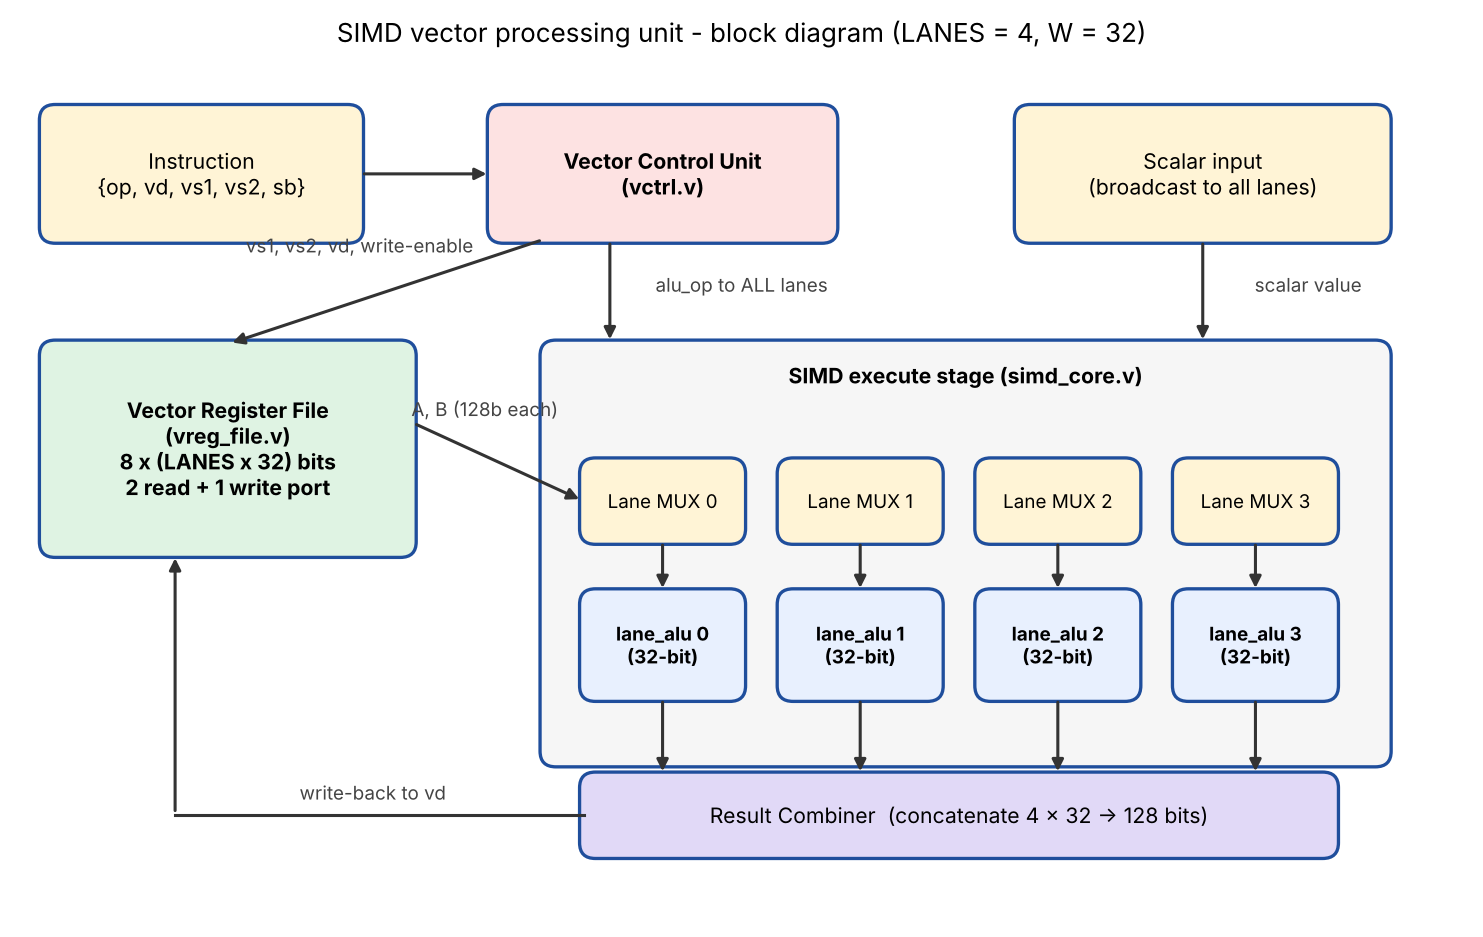
\includegraphics[width=\columnwidth]{block_diagram.png}
\caption{Block diagram of the SIMD unit ($L=4$, $W=32$).}\label{fig:block}
\end{figure}

\subsection{Instruction Set and Lane ALU}
Table~\ref{tab:isa} lists the operations. The opcode is used directly as the ALU operation, so the control unit needs no decode table. Comparisons return an all-ones lane value for true and zero for false, the mask convention of real SIMD hardware. Less-than is \emph{signed}, so $-1<1$ holds. Shift amounts use the low $\log_2 W$ bits of operand~B. Opcodes above 10 are no-operations and never write the register file.

\begin{table}[t]\centering\caption{Instruction set (opcode = ALU operation)}\label{tab:isa}
\begin{tabular}{@{}cll@{}}\toprule
Code & Mnemonic & Per-lane operation\\\midrule
0 & VADD & $a+b$\\ 1 & VSUB & $a-b$\\ 2 & VAND & $a\ \&\ b$\\ 3 & VOR & $a\ |\ b$\\ 4 & VXOR & $a\oplus b$\\
5 & VCMPEQ & $(a=b)$ ? all-ones : 0\\ 6 & VCMPLT & $(a<b)$ signed ? all-ones : 0\\
7 & VSLL & $a\ll b[4:0]$\\ 8 & VSRL & $a\gg b[4:0]$\\ 9 & VMUL & low 32 bits of $a\times b$\\ 10 & VMOV & $b$ (broadcast move)\\\bottomrule
\end{tabular}\end{table}

\subsection{Scalar Machine and Benchmark}
The workload is $C[i]=A[i]\ \mathrm{op}\ B[i]$ for $N=1024$ elements. Two independent machines run it on identical data.

\emph{Scalar machine} (\texttt{scalar\_top.v}): three 32-bit registers, one ALU (the same \texttt{lane\_alu} module used by the SIMD lanes) and a controller that moves one element per load. \emph{SIMD machine} (\texttt{bench\_top.v}): the SIMD core with $L$ lanes and memories that deliver one $L$-element vector per load. Both use the same four-state iteration (load A, load B, execute, store C) and the same accounting rule, which counts every clock from the start handshake until \texttt{done} rises. Hence scalar cycles equal $4N+1$ and SIMD cycles equal $4\lceil N/L\rceil+1$. Because the ALU, clock and loop structure are identical, the only difference between the machines is the number of elements handled per iteration. As a cross-check, the SIMD core with one lane reproduces the scalar cycle count exactly.

\subsection{Verification}
Each module has its own self-checking testbench with a behavioural golden model and automatic PASS/FAIL reporting. The lane ALU is tested exhaustively on an 8-bit instance (all $2^{16}$ operand pairs for all 11 operations, plus illegal opcodes) and with corner and random 32-bit vectors (753\,901 checks). The register file is tested for reset, isolation between registers, write-enable behaviour and read-during-write timing (1636 checks). The decoder is tested for all 16 opcodes (8000 checks). The system testbench applies directed, corner-case (0, all-ones, extreme values, signed overflow), random (2000 vectors per opcode), scalar-broadcast, lane-independence (perturb one lane, verify all others unchanged) and back-to-back read-after-write tests, and prints an opcode-by-test-type coverage matrix; it passes for 1, 2, 4 and 8 lanes (26\,525 to 65\,025 checks). The comparison testbench runs both machines on the same data for five operations and checks every element of both result arrays. To confirm the testbench is effective, six faults were injected deliberately (unsigned compare, wrong subtract, arithmetic instead of logical shift, lane crosstalk, illegal opcode writing, scalar multiplexer disabled); all six were detected.

\subsection{Experimental Setup}
Simulation: Icarus Verilog 12.0. Frequency and resources: Yosys 0.33 (\texttt{synth\_ecp5}) and nextpnr-ecp5 0.6 targeting a Lattice ECP5-85k model, 100\,MHz target clock, fixed seed. To keep the number of I/O pins small, the core is wrapped in a serial shift-register wrapper so the placed design contains all of the real logic. We used this open-source flow because a vendor tool (Vivado, Quartus) was not available; absolute frequencies on ECP5 are lower than on modern Xilinx or Intel devices, so the trend with lane count is the meaningful result.

\subsection{Results}
\textbf{Cycle count.} Table~\ref{tab:perf} gives simulated cycle counts on identical data. Speed-up is scalar cycles divided by SIMD cycles; efficiency is speed-up divided by lane count.

\begin{table}[t]\centering\caption{Scalar machine vs.\ SIMD machine, $N=1024$ (simulation)}\label{tab:perf}
\begin{tabular}{@{}rrrrr@{}}\toprule
Lanes & Scalar cyc. & SIMD cyc. & Speed-up & Efficiency\\\midrule
1 & 4097 & 4097 & 1.00$\times$ & 100\%\\
2 & 4097 & 2049 & 2.00$\times$ & 100\%\\
4 & 4097 & 1025 & 4.00$\times$ & 99.9\%\\
8 & 4097 & 513 & 7.99$\times$ & 99.8\%\\\bottomrule
\end{tabular}\end{table}

\textbf{Waveforms.} Fig.~\ref{fig:wave} shows the four lanes executing VADD, VSUB, VAND, signed VCMPLT, a scalar-broadcast VADD and two back-to-back dependent VADDs. Each lane produces its own result in the same cycle; in VCMPLT only lane~0 ($-1<1$) returns an all-ones mask; and the dependent adds read the previous result correctly (11, 22, 44, 88 in lane~0). Fig.~\ref{fig:timeline} compares scalar and 4-lane execution of a 16-element addition: the SIMD unit completes after 4 iterations (17 cycles) versus 16 iterations (65 cycles).

\begin{figure*}[t]\centering
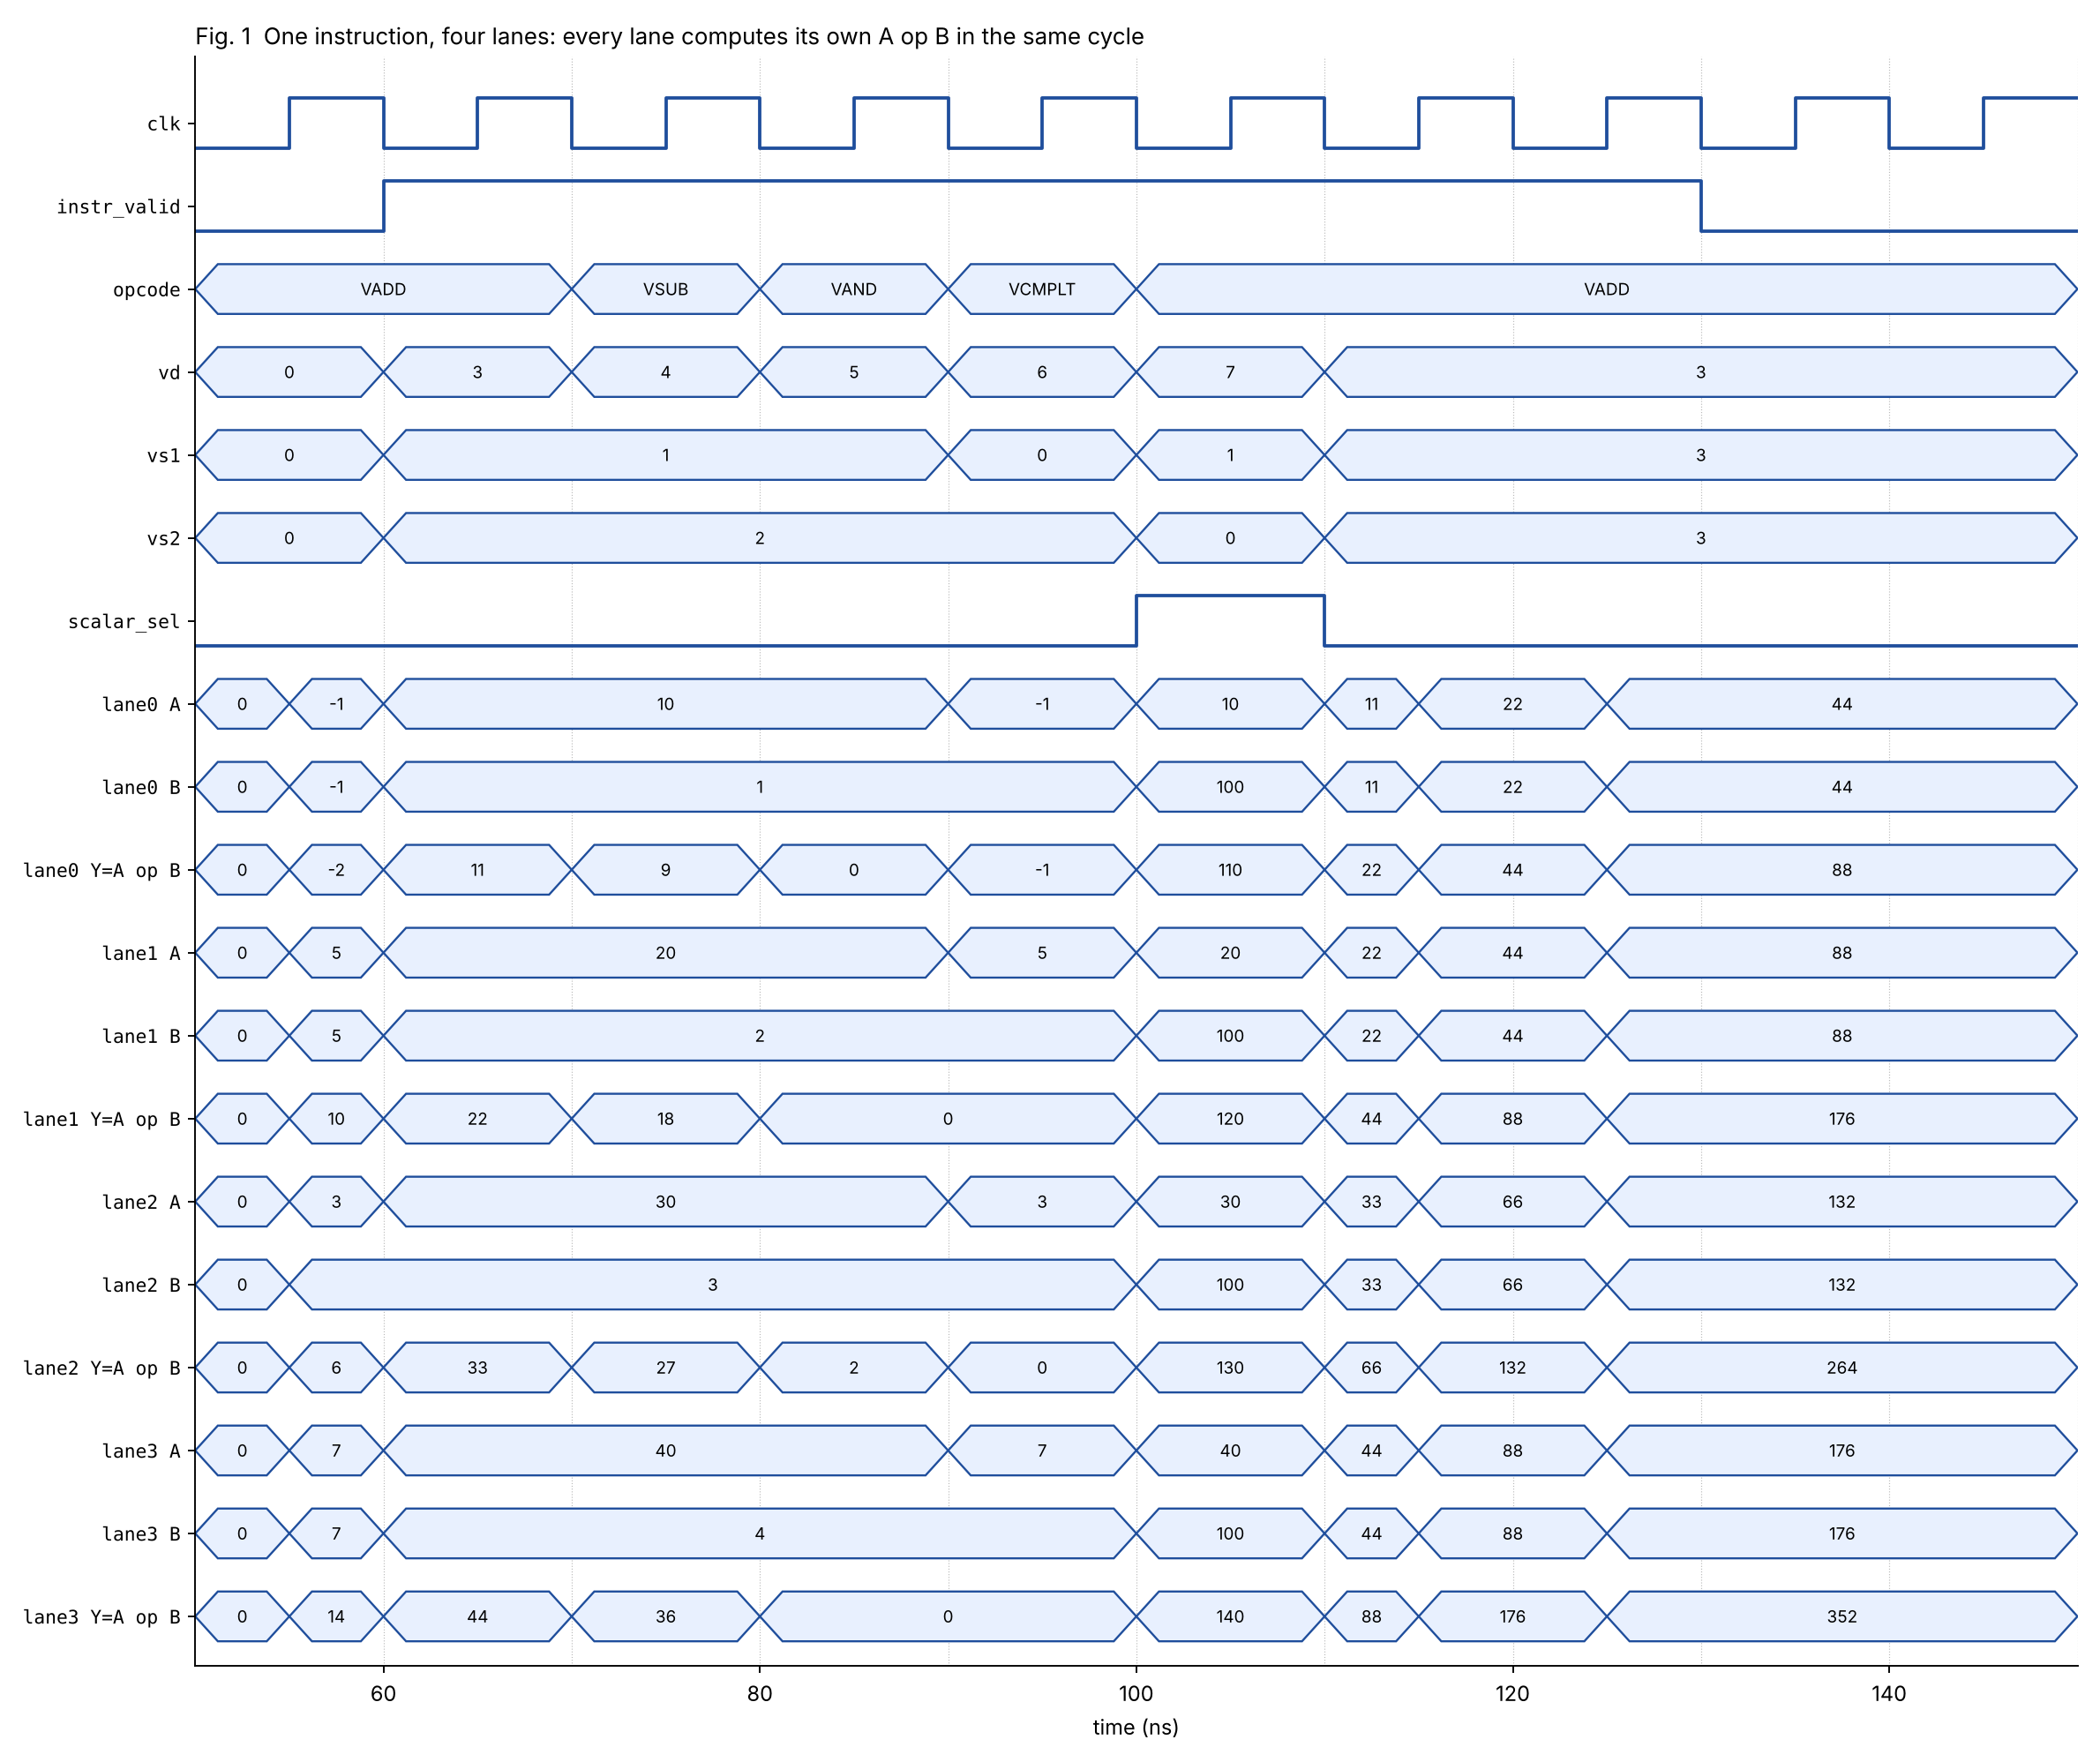
\includegraphics[width=0.86\textwidth]{fig1_parallel_lanes.png}
\caption{Simulation waveform: one instruction drives four lanes in parallel (generated from the testbench VCD).}\label{fig:wave}
\end{figure*}

\begin{figure}[t]\centering
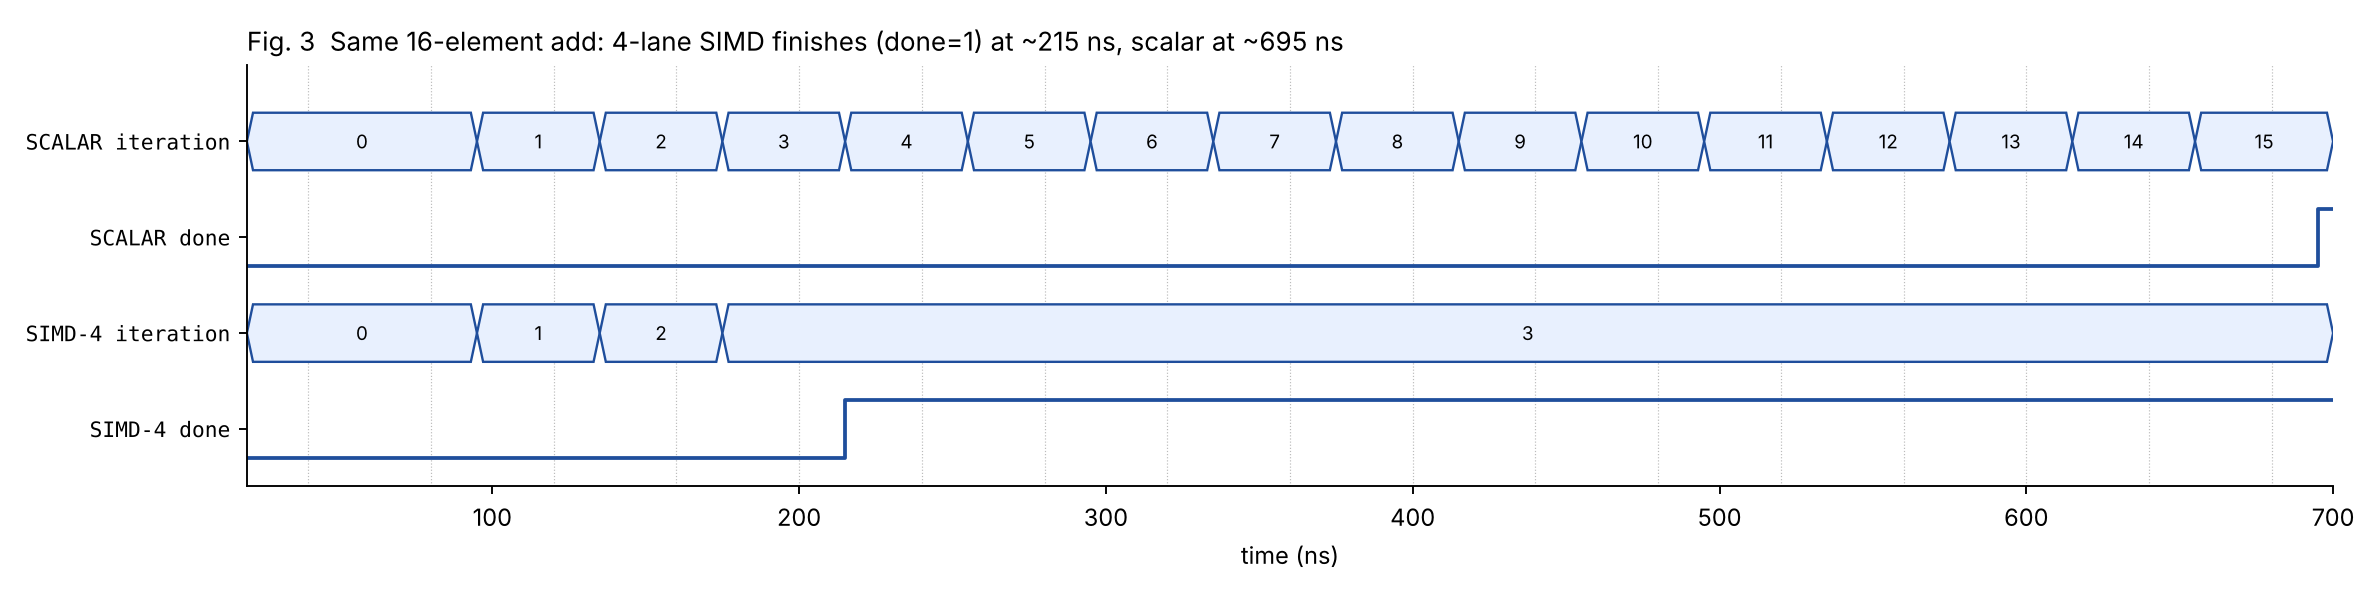
\includegraphics[width=\columnwidth]{fig3_scalar_vs_simd_timeline.png}
\caption{Scalar versus 4-lane SIMD on a 16-element addition.}\label{fig:timeline}
\end{figure}

\textbf{Frequency, throughput and area.} Table~\ref{tab:fmax} combines the cycle counts with the maximum frequency from place-and-route. Execution time is cycles divided by frequency; throughput is $N$ divided by execution time. The scalar reference uses the one-lane clock. The maximum frequency falls from 65.0\,MHz (1 lane) to 54.4\,MHz (8 lanes) because wider register-file read multiplexers, higher fan-out of the control signals and longer routing lengthen the critical path; consequently the time speed-up (3.74$\times$ for 4 lanes, 6.67$\times$ for 8) is lower than the cycle speed-up. Differences of one or two MHz, such as the 2-lane figure being slightly above the 1-lane figure, are placement noise from a single seed and should not be over-interpreted. LUTs, flip-flops and multiplier blocks grow almost linearly with lanes (Fig.~\ref{fig:chart}); flip-flops are dominated by the register file, whose width scales with $L$.

\begin{table*}[t]\centering\caption{Execution time, throughput and resources (ECP5-85k model, nextpnr; $N=1024$)}\label{tab:fmax}
\begin{tabular}{@{}rrrrrrrrr@{}}\toprule
Lanes & Cycles & Fmax (MHz) & Time ($\mu$s) & Throughput (M elem/s) & Time speed-up & LUT4 & FF & MULT18\\\midrule
1 (scalar ref.) & 4097 & 65.0 & 63.0 & 16.3 & 1.00$\times$ & 2490 & 375 & 3\\
2 & 2049 & 65.8 & 31.1 & 32.9 & 2.02$\times$ & 4400 & 695 & 6\\
4 & 1025 & 60.8 & 16.8 & 60.8 & 3.74$\times$ & 9068 & 1335 & 12\\
8 & 513 & 54.4 & 9.4 & 108.5 & 6.67$\times$ & 19\,526 & 2615 & 24\\\bottomrule
\end{tabular}\end{table*}

\begin{figure*}[t]\centering
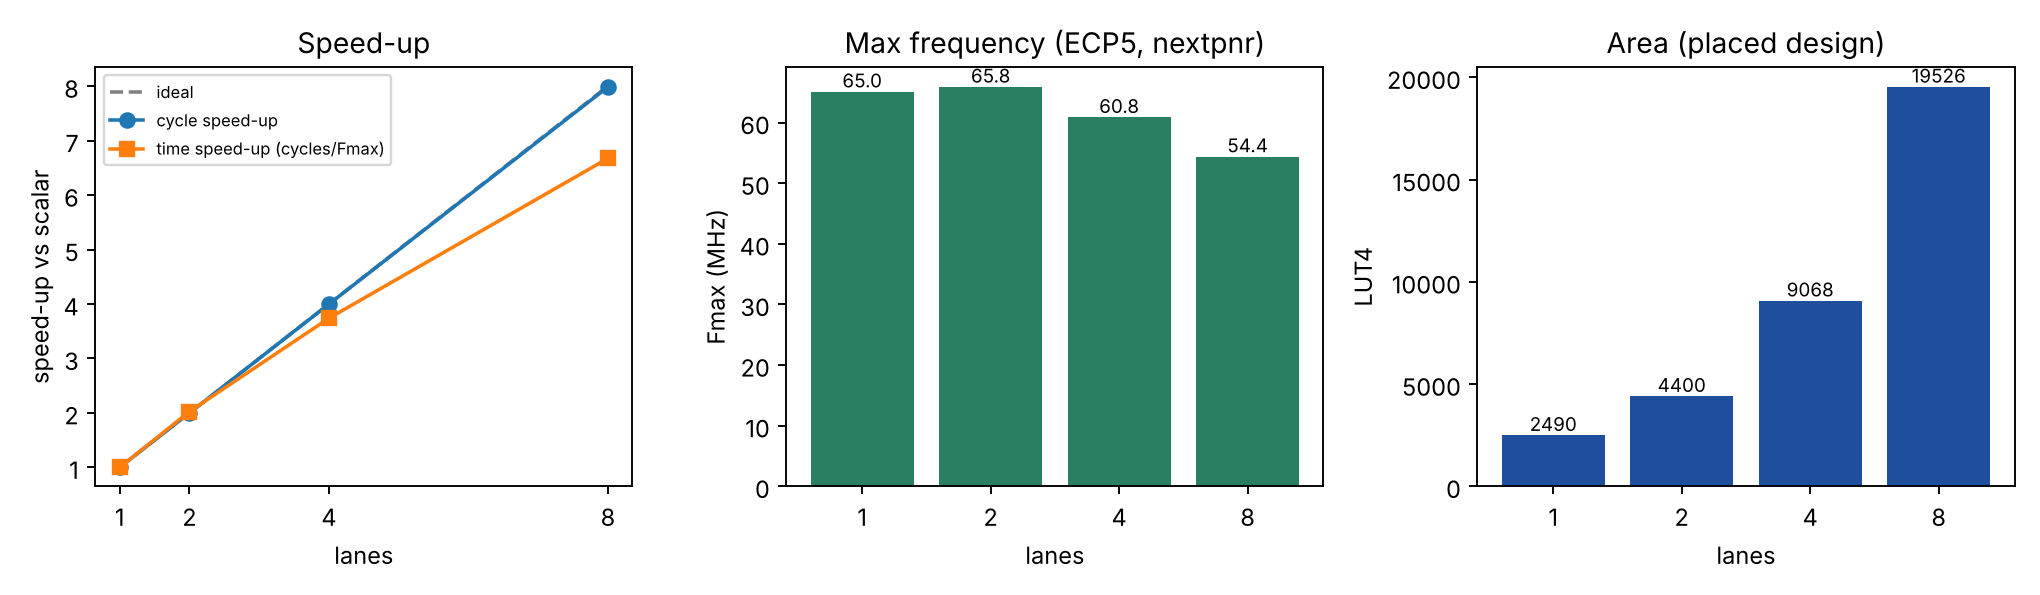
\includegraphics[width=0.85\textwidth]{results_chart.png}
\caption{Cycle and time speed-up, maximum frequency, and LUT usage versus number of lanes.}\label{fig:chart}
\end{figure*}

\subsection{Discussion and Limitations}
The cycle efficiency is close to 100\% because the benchmark loop has the same four-cycle structure for every lane count and the memory delivers one full vector per cycle, so memory bandwidth grows with the number of lanes. A real system with a fixed-width bus would be limited by memory, and loop overhead and non-vectorisable work would reduce the speed-up as described by Amdahl's law~\cite{amdahl1967}. When $N$ is not a multiple of $L$ the last vector is partly empty and the extra lanes do wasted work (the benchmark pads with zeros). The design is single-cycle, so its clock is set by read, ALU and write-back together; pipelining would raise the frequency. The scalar machine uses the one-lane core's frequency as its clock reference rather than being timed separately. Frequencies and areas come from an open-source flow on a different FPGA family than Xilinx or Intel and from one seed; they should be read as consistent relative measurements, and a vendor tool run would give different absolute values.

\subsection{Future Work}
Pipelining the execute stage; a vector-length register for arbitrary $N$; lane masking and predication; a narrower memory interface with strided access; and a vendor tool flow for absolute frequency on a Xilinx or Intel device.

\section{Individual Contributions}
Table~\ref{tab:contrib} lists what each member designed, tested and wrote. All members reviewed one another's code through GitHub pull requests.

\begin{table*}[t]\centering\caption{Contributions of each team member}\label{tab:contrib}
\renewcommand{\arraystretch}{1.2}
\begin{tabular}{@{}p{0.07\textwidth}p{0.30\textwidth}p{0.30\textwidth}p{0.22\textwidth}@{}}\toprule
Member & Design / code & Verification and results & Report sections\\\midrule
{[Member 1]} & Top-level integration \texttt{simd\_core.v} (generate-loop lanes, lane MUXes, result combiner, write-port arbitration); Makefile, CI workflow, repository set-up & Integration testing of the full core; final build and clean-clone run & Abstract, Introduction, Discussion, report assembly\\
{[Member 2]} & Lane ALU \texttt{lane\_alu.v} (11 operations, signed compare, masks); block-diagram script & \texttt{tb\_lane\_alu.v}: exhaustive 8-bit test (65\,536 pairs $\times$ 11 ops) and 32-bit corner/random tests & Section on instruction set and lane ALU; Fig.~\ref{fig:block}\\
{[Member 3]} & Vector register file \texttt{vreg\_file.v}; timing wrapper \texttt{fmax\_wrap.v}; \texttt{fmax.sh} open-source frequency/area flow & \texttt{tb\_vreg\_file.v}; Fmax and resource measurements for 1, 2, 4, 8 lanes & Literature review; Experimental setup; Table~\ref{tab:fmax} data\\
{[Member 4]} & Vector control unit \texttt{vctrl.v}; instruction format and ISA document & \texttt{tb\_vctrl.v}; system testbench \texttt{tb\_simd\_core.v} with golden model, lane-independence and RAW tests, coverage matrix; fault-injection (6 bugs) & Verification subsection\\
{[Member 5]} & Scalar machine \texttt{scalar\_top.v}; SIMD benchmark \texttt{bench\_top.v}; waveform and table/chart scripts & \texttt{tb\_bench.v}, \texttt{tb\_compare.v}, \texttt{tb\_waves.v}; cycle, speed-up, time and throughput analysis; waveform figures & Scalar machine and benchmark subsection; Results\\\bottomrule
\end{tabular}\end{table*}

\section*{Acknowledgment}
[Optional: thank the course instructor. If an AI assistant was used for code or text drafting, state it here as required by your course policy.]

\begin{thebibliography}{99}
\bibitem{flynn1966} M. J. Flynn, ``Very high-speed computing systems,'' \emph{Proc. IEEE}, vol. 54, no. 12, pp. 1901--1909, Dec. 1966.
\bibitem{flynn1972} M. J. Flynn, ``Some computer organizations and their effectiveness,'' \emph{IEEE Trans. Comput.}, vol. C-21, no. 9, pp. 948--960, Sep. 1972.
\bibitem{russell1978} R. M. Russell, ``The CRAY-1 computer system,'' \emph{Commun. ACM}, vol. 21, no. 1, pp. 63--72, Jan. 1978.
\bibitem{hennessy2019} J. L. Hennessy and D. A. Patterson, \emph{Computer Architecture: A Quantitative Approach}, 6th ed. Cambridge, MA, USA: Morgan Kaufmann, 2019.
\bibitem{peleg1996} A. Peleg and U. Weiser, ``MMX technology extension to the Intel architecture,'' \emph{IEEE Micro}, vol. 16, no. 4, pp. 42--50, Aug. 1996.
\bibitem{stephens2017} N. Stephens \emph{et al.}, ``The ARM Scalable Vector Extension,'' \emph{IEEE Micro}, vol. 37, no. 2, pp. 26--39, Mar./Apr. 2017.
\bibitem{riscvv} RISC-V International, ``RISC-V `V' Vector Extension, Version 1.0,'' 2021.
\bibitem{lindholm2008} E. Lindholm, J. Nickolls, S. Oberman, and J. Montrym, ``NVIDIA Tesla: A unified graphics and computing architecture,'' \emph{IEEE Micro}, vol. 28, no. 2, pp. 39--55, Mar./Apr. 2008.
\bibitem{yu2008} J. Yu, G. Lemieux, and C. Eagleston, ``Vector processing as a soft-core CPU accelerator,'' in \emph{Proc. ACM/SIGDA Int. Symp. Field-Programmable Gate Arrays (FPGA)}, 2008, pp. 222--232.
\bibitem{yiannacouras2008} P. Yiannacouras, J. G. Steffan, and J. Rose, ``VESPA: Portable, scalable, and flexible FPGA-based vector processors,'' in \emph{Proc. Int. Conf. Compilers, Architectures and Synthesis for Embedded Systems (CASES)}, 2008, pp. 61--70.
\bibitem{amdahl1967} G. M. Amdahl, ``Validity of the single processor approach to achieving large scale computing capabilities,'' in \emph{Proc. AFIPS Spring Joint Comput. Conf.}, 1967, pp. 483--485.
\end{thebibliography}
\end{document}
